\documentclass[10pt,xcolor=pdflatex, notes=only]{beamer}
%\documentclass[10pt,xcolor=pdflatex]{beamer}
\usepackage{newcent}
\usepackage[utf8]{inputenc}
\usepackage[czech]{babel}
\usepackage{graphicx}
\usepackage{animate}
\usepackage{hyperref}
\usepackage{fancyvrb}
\usetheme{FIT}

\graphicspath{{./img/}}

\setbeamerfont{note page}{size=\tiny}

%%%%%%%%%%%%%%%%%%%%%%%%%%%%%%%%%%%%%%%%%%%%%%%%%%%%%%%%%%%%%%%%%%
\title[Komponentní systém]{Komponentní systém pro herní grafický engine}

\author[]{Tomáš Polášek}

\institute[]{Vysoké Učení Technické v Brně, Fakulta Informačních Technologií\\
Bo\v{z}et\v{e}chova 1/2. 612 66 Brno - Kr\'alovo Pole\\
xpolas34@fit.vutbr.cz}

\date{16. června 2017}
%\date{\today}
%\date{} % bez data

%%%%%%%%%%%%%%%%%%%%%%%%%%%%%%%%%%%%%%%%%%%%%%%%%%%%%%%%%%%%%%%%%%

%\begin{document}

%\frame[plain]{\titlepage}

%\begin{frame}\frametitle{Frame Title}
%    Example \emph{content}.
%\end{frame}

%\bluepage{Thank You For Your Attention !}

%\end{document}
\begin{document}
	
\frame{\titlepage}
	
\begin{frame}
	\frametitle{Cíle práce}
	\begin{itemize}
		\item Návrh a implementace entitního systému
		\item Priority:
		\begin{enumerate}
			\item Paralelní přístup
			\item Modularita a přizpůsobitelnost
			\item Optimalizace 
		\end{enumerate}
	\end{itemize}
\end{frame}

\note{
	Cílem této bakalářské práce byl návrh a implementace entitního systému založeného na kompozici, se zaměřením na využití v herních grafických enginech.
	\begin{itemize}
		\item Návrh a implementace entitního systému = Založeného na kompozici, zaměření na použití v herních grafických enginech.
		\item Priority: = V práci jsem se dále soustředil na 
			\item \#Paralelní přístup = Umožnení paralelního přístupu k výslednému systému.
			\item \#Modularita a přizpůsobitelnost = Protože jsou herní enginy téměř vždy specializované na určitý typ her, bylo důležité Další prioritou byla modularita a přizpůsobytelnost.
			\item \#Optimalizace využití RVP = Důležitou částí byly také optimalizace, primárně ve směru efektivního využití rychlých vyrovnávacích pamětí
	\end{itemize}
	1 minuta
}

\begin{frame}[t]
\frametitle{Význam}
\begin{itemize}
	\item Jádro herního enginu
	\begin{itemize}
		\item Komunikace mezi moduly
		\item Omezující faktor
	\end{itemize}
	\item Nedostatky aktuálních řešení
	\begin{itemize}
		\item Akumulace nechtěného stavu
		\item Komunikace mezi entitami
		\item Omezené množství typů
	\end{itemize}
	\item \emph{Entity-Component-System} paradigma
\end{itemize}
	\vfill
	\begin{center}
		\includegraphics[width=0.6\textwidth]<2->{ECS1}
	\end{center}
	\vfill
\end{frame}

\note{
	Dále bych přešel k důvodům, proč jsem si toto téma vybral a proč je důležité tuto problematiku řešit.
	\begin{itemize}
		\item Jádro grafického enginu = Entitní systém je jádrem herního enginu, který zprostředkovává komunikaci mezi jednotlivými moduly. Tímto však na něm vzniká de facto závislot, která může být v dalším vývoji problmatická. Je tedy nutné navrhnout entitní systém tak, aby zbytečně zbytek herního enginu neomezoval.
		\item Nedostatky aktuálních řešení = Tím se dostávám k dalšímu bodu, čímž jsou nedostatky aktuálních řešení založených na dědičnosti. Mezi ně patří například:
			\item -Akumulace stavu a chování = Při průchodu stromu dědičnosti
			\item -Komunikace mezi entitami = Dalším problémem je komunikace
			\item -Neohebnost typů = Omezená množina typů, vytvořená programátorem ve zdrojovém kódu.
		\item \emph{Entity-Component-System} paradigma = Dalším bodem je ECS paradigma, na kterém je tato práce založena. ECS je programovací paradigma založené na kompozici a vzniká z objektové orientace. Mezi základní pojmy patří Entita, Komponent a Systém. ECS lze přirovnat k tabulce v databázi, kde sloupce reprezentují jednotlivé komponenty a řádky entity.
	\end{itemize}
	2 minuty
}

\begin{frame}
	\frametitle{Řešení I}
	\begin{itemize}
		\item Dekompozice problému
		\item Entita = Identifikátor + metadata
		\item Komponenty
		\begin{itemize}
			\item Pasivní datová struktura
			\item Individuální nosiče
		\end{itemize}
		\item Systémy 
		\begin{itemize}
			\item Skupiny entit
		\end{itemize}
		\item Paralelní zpracování
		\begin{itemize}
			\item Entitní
			\item Systémový
			\item Množiny změn
		\end{itemize}
	\end{itemize}
\end{frame}

\note{
	Tímto se dostávám k samotnému návrhu entitního systému.
	Předpoklady - mnozina se kterou se pracuje, specifika podle zamereni enginu
	\begin{itemize}
		\item Dekompozice problému = Základem byla dekompozice problému do pěti modulů, o jejichž funkci se nyní ve zkratce zmíním.
		\item Entita = Identifikátor + metadata = První z nich je správa entit a jejich metadat. Entity jsou reprezentovány celočíselným identifikátorem a mají přidělený řádek v tabulce metadat. 
		\item Komponenty = Další doménou jsou komponenty a jejich nosiče. Komponentou může být libovolná pasivní datová struktura, přičemž by něměla obsahovat žádné výkonné operace. Zajímavou částí jsou nosiče komponent. Nosičem je datová struktura, která udržuje mapování komponenty daného typu na entitu. Každá komponenta může mít definovaný svůj typ nosiče, což umožňuje vyšší specializaci entitního systému.
			\item -Pasivní datová struktura
			\item -Individuální nosiče
		\item Systémy = Doména systémů je ve skutečnosti rozdělena do dvou - samotné systémy a entitní skupiny. Každý systém specifikuje komponenty o které má zájem. Každému systému je přiřazena skupina entit, která zaručeně obsahuje pouze takové entity, o které má systém zájem. Tímto je umožněna nepřerušená iterace nad entitami, bez nutnosti opakovaného testování.
			\item -Specifikace komponent
			\item -Skupiny entit
		\item Paralelní zpracování = Poslední částí je modul paralelního zpracování. Součástí návrhu jsou tři způsoby paralelizmu - entitní, systémový a pomocí množin změn. Cílem tohoto modulu je údržba a následná aplikace množin změn.
	\end{itemize}
	3 minuty
}

\begin{frame}
	\frametitle{Řešení II}
	\begin{itemize}
		\item Fáze operace 
		\begin{enumerate}
			\item Inicializace
			\item Iterace
			\item Obnova
		\end{enumerate}
		\item Implementační jazyk C++
		\begin{itemize}
			\item Generické programování
			\item Generování kódu
		\end{itemize}
		%\item Tabulka metadat
		%\begin{itemize}
		%	\item Identifikátor = Generace + Index
		%	\item Horizontální x Vertikální
		%\end{itemize}
	\end{itemize}
	%\vspace{0.5em}
	\vfill
	\begin{center}
		%\includegraphics[width=0.6\textwidth]<2>{identifier}
		%\includegraphics[width=\textwidth]<3>{metadata}
	\end{center}
	\vfill
\end{frame}

\note{
	\begin{itemize}
		\item Fáze operace = Dalším bodem této prezentace jsou jednotlivé fáze, ve kterých se může entitní systém nacházet.
			\item -Inicializace = První z nich je fáze inicializace, ve které jsou registrovány komponenty, které budou následně použivány.
			\item -Iterace = Následuje fáze iterace, která umožňuje plný přístup k entitnímu systému
			\item -Obnova = Poslední fází, do které lze přejít po dokončení iterace, je obnova. Součástí obnovy je dokončení zpožděných operací a uvedení entitního systému do konzistentního stavu.
		\item Implementační jazyk C++ = Pro implementaci byl zvolen programovací jazyk C++, který je standardem při vývoji herních enginů. Kromě jeho základních vlastností bylo také využito generického programování za pomocí šablon. Dále bylo také využito metaprogramování ke generování kódu.
			\item -Generické programování
			\item -Generování kódu
			\item -Data Oriented Design
		%\item Tabulka metadat = Zajímavým problémem byla tabulka metadat, kdy bylo nutné určit jaké informace bude obsahovat a jakým způsobem bude reprezentována.
		%\begin{itemize}
			%\item Identifikátor = Generace + Index = Nejdříve je nutné specifikovat identifikátor, který byl rozdělen na dvě části. Index, který operuje jako ukazatel do tabulky metadat a generace, která umožňuje rozpoznávat různé entity, na stejném řádku tabulky - např. smazané. Tabulka tedy obsahuje aktuální generaci každého řádku. Kromě toho obsahuje také značku o přítomnosti různých typů komponent a přítomnost dané entity ve skupinách entit. Tyto informace jsou dále využity při optimalizacích.
			%\item Horizontální x Vertikální = Jelikož většina informací je typu přitomný/nepřítomný, je možné je reprezentovat pomocí bitů. Zde však nastává problém, protože operace nad množinou bitů nejsou atomicke. Toto lze vyřešit vertikální orientací jednotlivých bitových množin.
		%\end{itemize}
	\end{itemize}
}

\iffalse

%\begin{frame}[t]
	\frametitle{Paralelizmus}
	\begin{columns}[t, onlytextwidth]
		\begin{column}{0.5\textwidth}
			\begin{itemize}
				\item Minimalizace zámků
				\item Podporované typy:
				\begin{enumerate}
					\item Entitní
					\item Systémový
					\item Množiny změn
				\end{enumerate}
				\item Transformace stavu
				\item Dočasné entity
			\end{itemize}
		\end{column}
		\begin{column}{0.5\textwidth}
			\begin{center}
				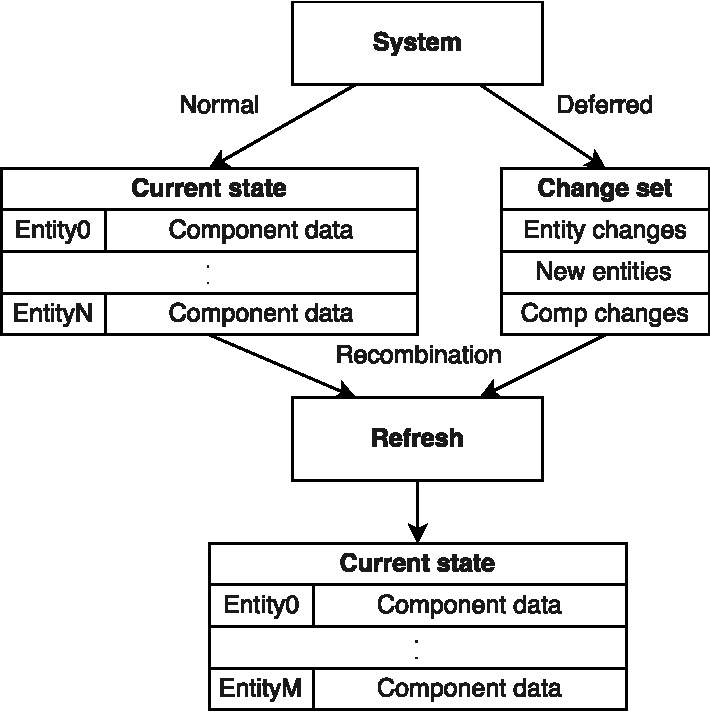
\includegraphics[width=\textwidth]{parallelism}
			\end{center}
		\end{column}
	\end{columns}
%\end{frame}

\fi

\begin{frame}
	\frametitle{Výsledky}
	\begin{itemize}
		\item Multiplatformní knihovna \textbf{Entropy}
		\item Optimalizace
		\item Podpora paralelizmu
		\item Třídní rozhraní
		\item Možnosti rozšíření
		\begin{itemize}
			\item Paralelizace obnovovací fáze
			\item Serializace entit
			\item Vazba na skriptovací jazyky
			\item Předlohy entit
			\item Dynamické komponenty
		\end{itemize}
	\end{itemize}
\end{frame}

\note{
	Na závěr bych rád znovu shrnul hlavní výsledky této bakalářské práce.
}

\begin{frame}
	\frametitle{Závěr}
	\begin{center}
		%\animategraphics[loop, autoplay, width=\linewidth]{60}{animation-}{0}{762}
		%\animategraphics[loop, autoplay, width=\linewidth]{60}{animation-}{0}{700}
	\end{center}
\end{frame}

\end{document}